\documentclass[12pt,b5paper]{article}
\usepackage[utf8]{inputenc}
\usepackage{amsmath}
\usepackage{amsfonts}
\usepackage{amssymb}
\usepackage{graphicx}
\usepackage{lmodern}
\usepackage{fancyhdr}
\usepackage[left=2cm,right=2cm,top=2cm,bottom=0.5cm]{geometry}
\pagestyle{fancy}
\lhead{IFNTI Sokodé - Rapport BD}
\rhead{Novembre 2023}
\cfoot{\vspace{-5cm} Institut de Formation aux Normes de Technologie et de l'Informatique \\ 300 BP 40, Sokodé TOGO -- Tel 90 91 81 41}
\rfoot{\thepage}
\author{sankara sarata DEGBEBIAN Aïmane}
\begin{document}

\begin{center}
\textbf{INTRODUCTION}\\
\end{center}
Les fonctions SQL exécutent une liste arbitraire d'instructions SQL,renvoyant le résultat de la dernière requête de la liste.Dans la suite nous allons manipuler les fonctions SQL.Après nous allons créer deux tables dont l'identifiant de la seconde table  aura pour type le nom de la première table.
\section{Création des fonctions SQl}
\subsection{Création des la base de donnée}
Dans cette partie nous avons crée une base de donnée  ifnti qui a pour tables etudiant et enseignant\\

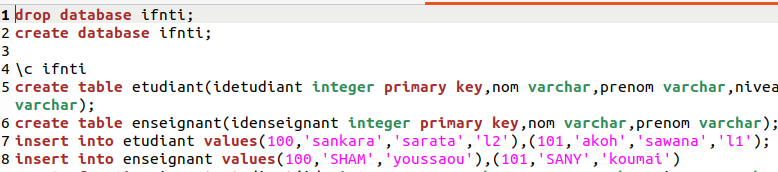
\includegraphics[scale=0.5]{ifnti}
\subsection{Création des fonctions sql}
\subsubsection{Création des fonctions sql ayant pour type de retour void}
Pour créer une fonction sql ayant pour type de retour void on utilise la syntaxe suivante \textbf{CREATE FUNCTION 	function\_name() returns void as ' '.} Cette fonction ne retourne rien.\\
Voici notre première tentative de création de la fonction insert-etudiant\\ 
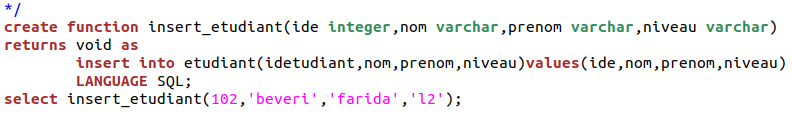
\includegraphics[scale=0.5]{er1}
Une erreur de syntaxe est engendré car nous avons omis les cotes \textbf{('')} entre le \textbf{as} et \textbf{language sql}. 
\newpage
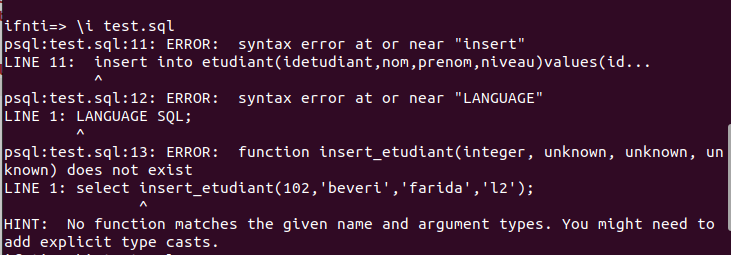
\includegraphics[scale=0.5]{erreur_insert_etudiant}\\
Pour corriger cette erreur nous avons mis les cotes \textbf{('')} entre le \textbf{as} et \textbf{language sql}.

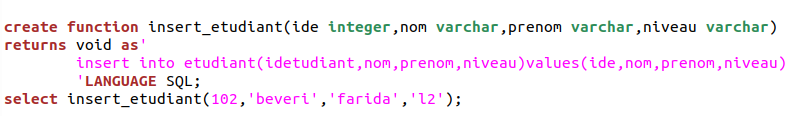
\includegraphics[scale=0.5]{fonc}\\

Après l’exécution nous avons obtenus le résultat suivant\\
\begin{center}
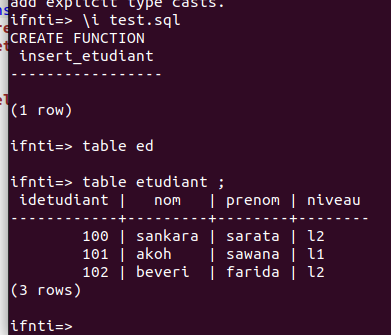
\includegraphics[scale=0.5]{insert_etudiant}

\end{center}
\subsubsection{Les fonctions ayant pour type de retour une ligne}
Les fonctions SQL peuvent prendre des paramètres en entré et retourner une seule ligne.Pour déclarer les paramètres on écrit le nom du paramètre suivit de son type mais pour le retour nous précisions le type de retour\newpage

.Exemple 1:Nous allons crée une fonction qui ne prend rien en paramètre et retourne une chaîne\\

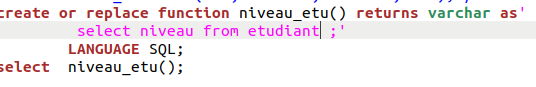
\includegraphics[scale=0.5]{var}\\
\begin{center}
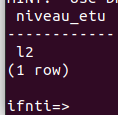
\includegraphics[scale=0.6]{res}\\
\end{center}
Exemple 2:Nous allons crée une fonction qui prend l'identifiant d'un enseignant en paramètre et retourne son nom qui est une chaîne\\

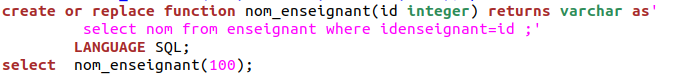
\includegraphics[scale=0.6]{nom_}\\
\begin{center}
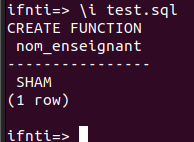
\includegraphics[scale=0.6]{ensei}\\

\end{center}
\subsection{Fonctions SQL avec des paramètres en sortie}
Nous pouvons définir des fonctions sql dont sont type de retour  est indiqué dans les paramètres .Pour declarer un paramètre en sortie on utilise le mot-clé \textbf{OUT}  et les paramètres en entrés est précéder de du mot-clé \textbf{IN}.Le mot-clé IN est optionnel et le OUT est obligatoire
exemple 1\\
\newpage
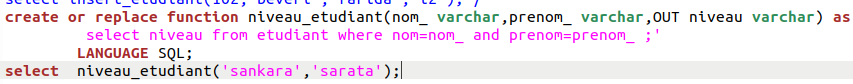
\includegraphics[scale=0.5]{out}\\

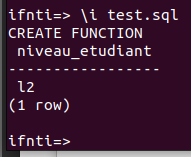
\includegraphics[scale=0.6]{out1}\\
Une erreur est produite parce que nous avons pas précisé le paramètre de retour donc en appelant la fonction il réclame trois arguments.

exemple 2\\
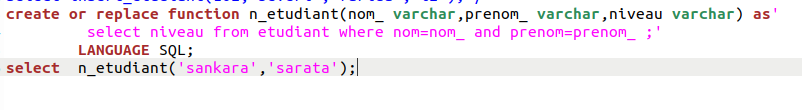
\includegraphics[scale=0.6]{out2}\\
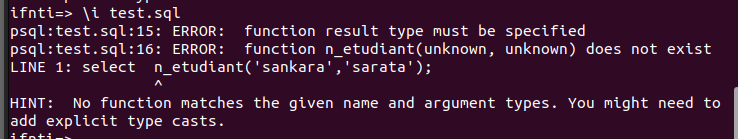
\includegraphics[scale=0.6]{out3}\\

\subsection{Création d'une fonction sql ayant pour type de retour \textbf{SETOF sometype}}

Le type de retour \textbf{SETOF sometype} nous permet de retourner plusieurs lignes mais nous avons remarqué le sometype est derivé par le nom de la table et il retourne tous les attributs de la de table.\\

Nous avons fait une premiere tentative en essayant de sélectionné les noms et les prénoms des étudiants.\\
 \newpage

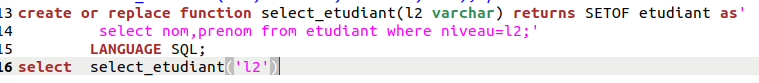
\includegraphics[scale=0.5]{ca}\\
 une erreur de retour a été engendré,il est impossible de sélectionner les colonnes d'une table avec le retour \textbf{SETOF}.\\
 
 
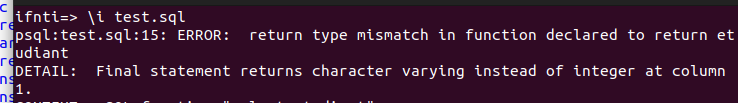
\includegraphics[scale=0.5]{erreur_setop}\\

Pour corriger cette erreur nous avons été obligée de sélectionnée tous les colonnes de la table.\\
 
 
 
 
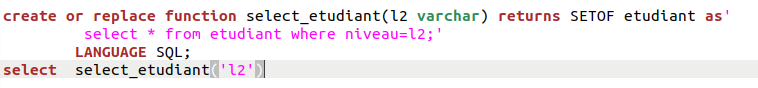
\includegraphics[scale=0.5]{select}\\

 Après l’exécution nous avons obtenus le résultat suivant:
 
\begin{center}
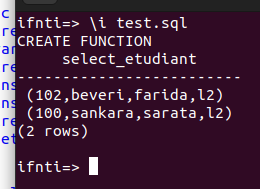
\includegraphics[scale=0.5]{resul_setof}\\
\end{center}
\newpage
\section{ Fonctions SQL renvoyant TABLE}
Dans Une fonction sql nous pouvons  retourner un ensemble de ligne avec syntaxe RETURNS TABLE(colonnes).\\ 

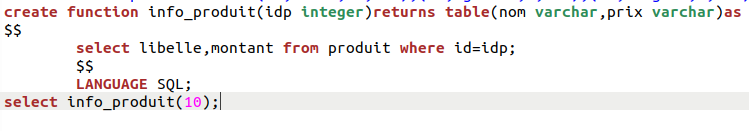
\includegraphics[scale=0.5]{pr}\\
\begin{center}
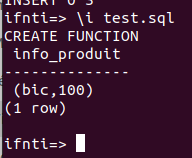
\includegraphics[scale=0.5]{pro}\\

\end{center}


\section{Créons les tables personne client }
Dans cette partie nous allons crée une table personne(idpersonne,nom,prenom) et une table client(identifiant,adresse)\\
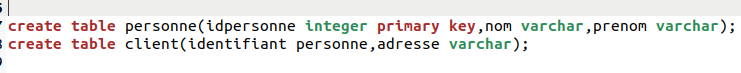
\includegraphics[scale=0.5]{tables}\\
\begin{center}
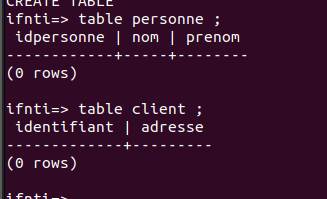
\includegraphics[scale=0.5]{ta}\\
\end{center}
\section{Inserons dans les tables personne et clients}

Pour faire l'insertion dans une table ayant pour colonne un type composite on ouvre les parenthèses pour saisir les champs correspondant et les séparez par des virgules.

Pour mettre un attribut vide on met les parenthèses du type composite entre guillemets unique et virgule .
Pour mettre un attribut la valeur null on met les parenthèses du type composite entre guillemets unique et guillemets doubles  pour la valeur nulle et les champs type chaîne.

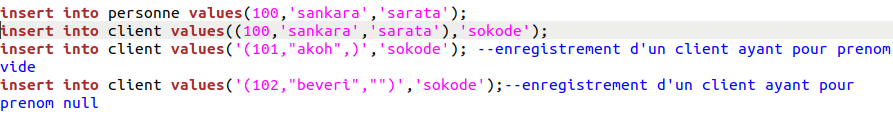
\includegraphics[scale=0.5]{in}\\
\newpage
\begin{center}
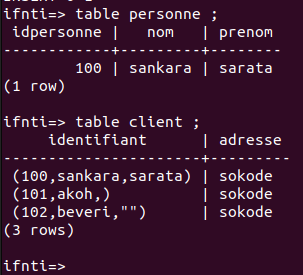
\includegraphics[scale=0.5]{t}\\
\end{center}
\section{Accéder aux types composite }
Pour accéder à un champ d'une colonne composite on écrit le nom de colonne point le nom  du champ ou (table-name.colonne-composite-name.nom-champ).notons bien le nom de colonne doit être toujours entre parenthèse .exemple

\textbf{select (identifiant).nom from client;}
\begin{center}
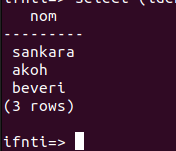
\includegraphics[scale=0.5]{nom}\\
\end{center}

\textbf{select (client.identifiant).prenom from client;}
\begin{center}
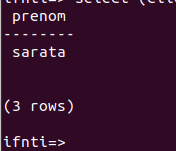
\includegraphics[scale=0.5]{pre}\\
\end{center}

\section{ Surcharge des fonctions}



\end{document}
